\chapter{ПЗУ}

\begin{center}
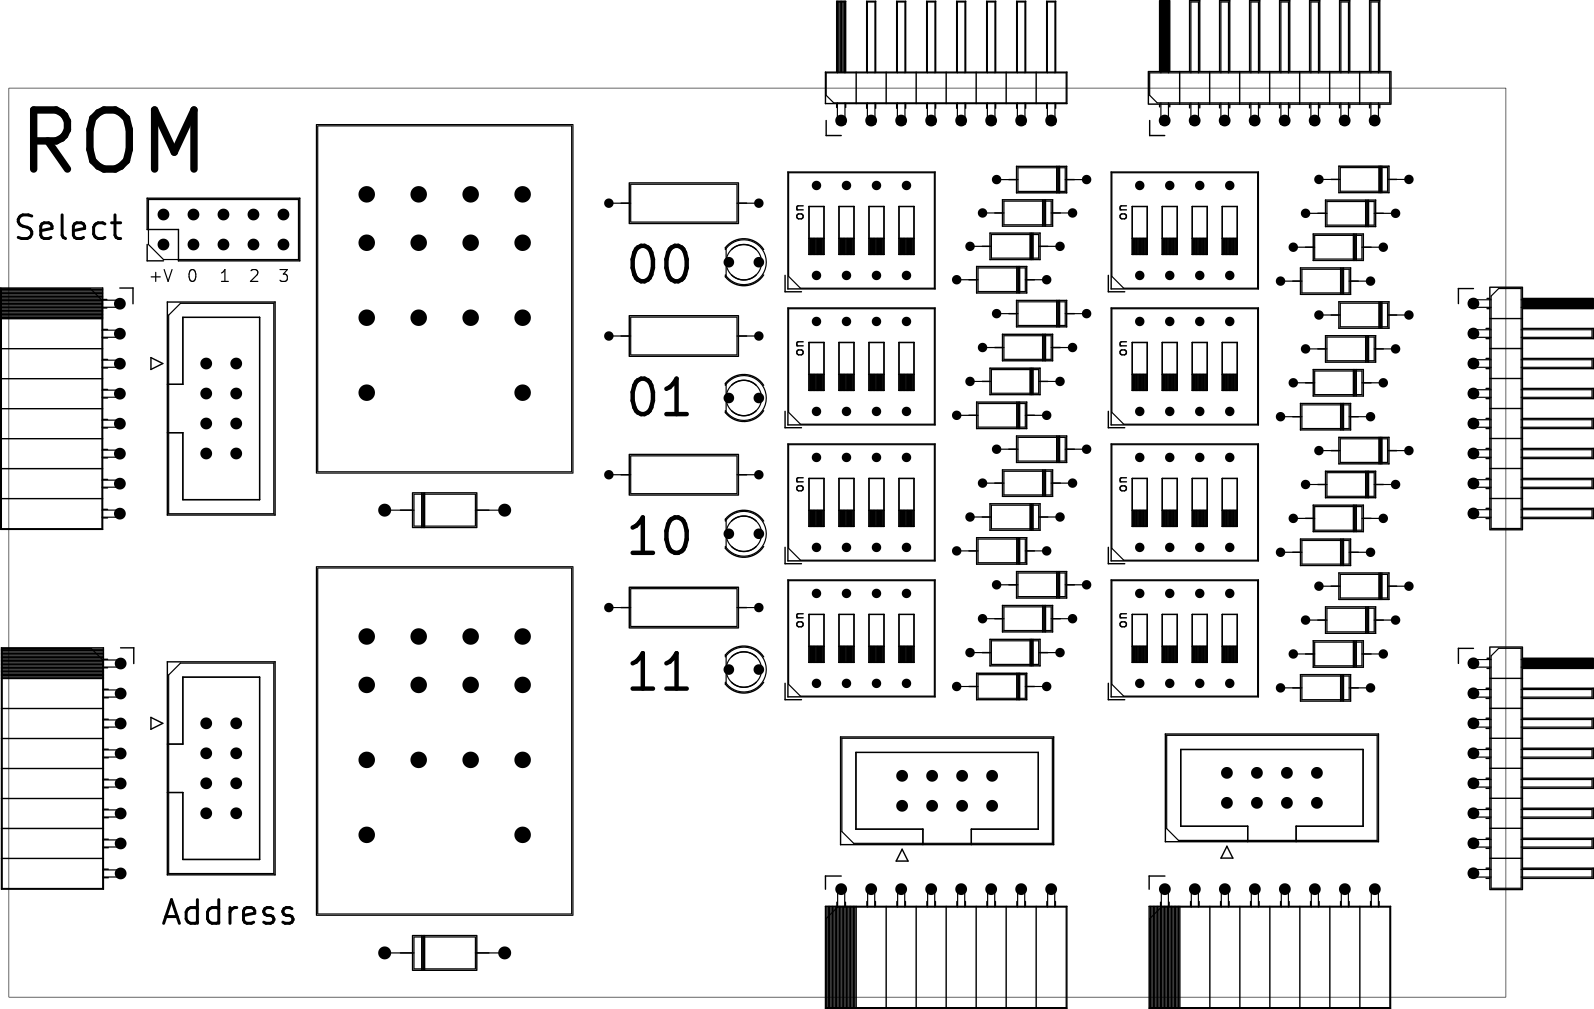
\includegraphics{../modules-png/rom-pcb.png}
\end{center}

\begin{center}
\includegraphics[width=0.5\columnwidth]{../modules-3d/rom.png}
\end{center}

\section{Практикум}

Список модулей:
\begin{itemize}
    \item ПЗУ: \modulesrom{1} штука
    \item Модуль переключателей: \modulesswitches{1} штука
    \item Модуль унарных операций: \modulesunary{1} штука
\end{itemize}

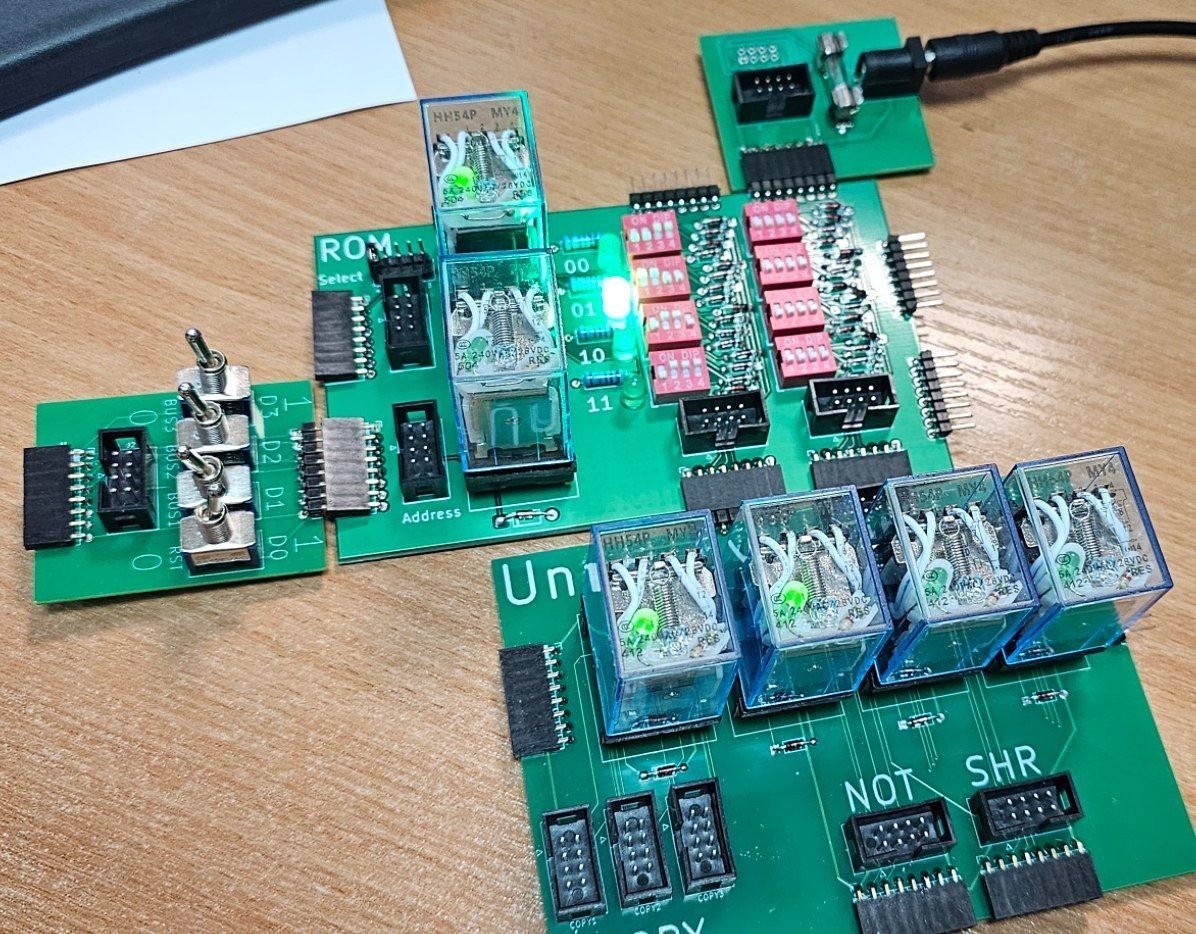
\includegraphics[width=0.5\columnwidth]{photo/rom.jpg}

\begin{enumerate}
    \item <<Запрограммируйте>> разные переключатели модуля ПЗУ на разные значения.
          Например, переключатели в верхнем ряду могут быть установлены в $0110$ и $0011$.
    \item Установите переключатели в положение $0000$.
    \item Модуль унарных операций должен отобразить значение $0110$, если подключен к левой шине и $0011$,
          если подключен к правой.
    \item Проверьте, что для других положений тумблеров значения из ПЗУ также считываются корректно.
    \item Переставьте модуль унарных операций на соседнюю шину и так же проверьте её работу.
\end{enumerate}

